\documentclass{article}
\usepackage{graphicx}
\raggedbottom
\begin{document}

\title{Mobile network signal strength in Makerere University.}
\date{20-May-2017}

\author{AYIKO JEREMIAH SARA}


\maketitle
\newpage

\begin{abstract}
Many students need to connect to the internet for personal and study purposes in Makerere University. Network across the University is a big factor in smooth access for the students. Data was collected from locations across the university. It was found out that network across the university was good however there were some poor signal zones. Students have sufficient network for reliable data connection.
\end{abstract}

\newpage

\tableofcontents
\newpage

\section{Intoduction}
A mobile network or cellular network is a communication network where the last link is wireless. The network is distributed over land areas called cells, each served by at least one fixed-location transceiver, known as a cell site or base station. This base station provides the cell with the network coverage which can be used for transmission of voice, data and others. A cell might use a different set of frequencies from neighboring cells, to avoid interference and provide guaranteed service quality within each cell.\cite{key:1}

\subsection{Background}
Following the recent surge in internet usage in Africa; between 2000 and 2017 the growth rate in Africa is 7,557.2\%\cite{key:2}, access to the internet has been critical to students to complement their class work. This has been done through research online, access to tutorials and books, etc. At Makerere University, students are mostly known to use internet for socialmedia. This has been attributed to high internet access costs and poor network coverage. This research will provide data for the signal strength of mobile networks in the university. It can be used by telecom companies to verify actual signal strengths in the university compared to signal sent from the transmission towers in order to boost network coverage within the university. The university itself can provide cellular network repeaters to boost signals within its faculties and halls of residence to allow smooth network access by students.

\section{Methodology}
The research will be carried out individually. I will develop a data collection electronic form using Open Data Kit (ODK). Then build the Aggregate server using the Google AppEngine platform thus creating an electronic data collection system. Then determine the locations for data collection within the university and collect data from those locations using the system that will be installed on my phone. The network signals will be collected using my phone which has a reading of network signal.

\section{Results}
The research was carried out between 7th May 2017 and 20th May 2017. Research planning and design started on 7th to 16th. Data collection was carried out from 17th to 19th. Analysis and report of findings carried out on 20th.

\subsection{Findings}
\begin{itemize}
\item
Figure 1: Data collected from device.
\item
Figure 2: More data collected from device.
\item
Figure 3: Bar graph of HSPA+  network locations and signal strength.
\item
Figure 4: Bar graph of HSPA  network locations and signal strength.
\item
Figure 5: Bar graph of EDGE  network locations and signal strength.
\item
Figure 6: North part of the university with network signals.
\item
Figure 6: Middle part of the university with network signals.
\item
Figure 6: South part of the university with network signals.
\end{itemize}
	
\begin{figure}
  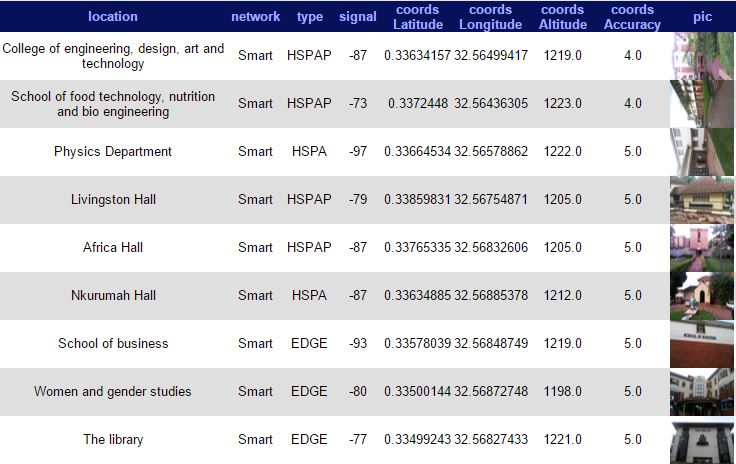
\includegraphics[width=\linewidth]{tableone.jpg}
  \caption{Data Table (a)}
  \label{fig:dt1}
\end{figure}

\begin{figure}
  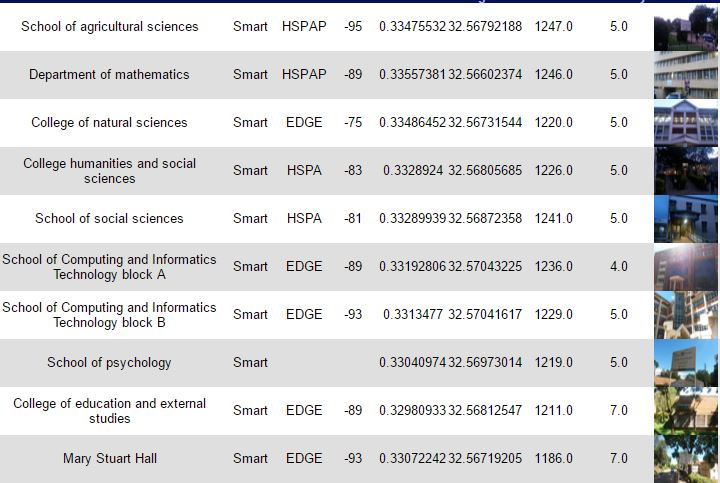
\includegraphics[width=\linewidth]{tabletwo.jpg}
  \caption{Data Table (b)}
  \label{fig:dt2}
\end{figure}

\begin{figure}
  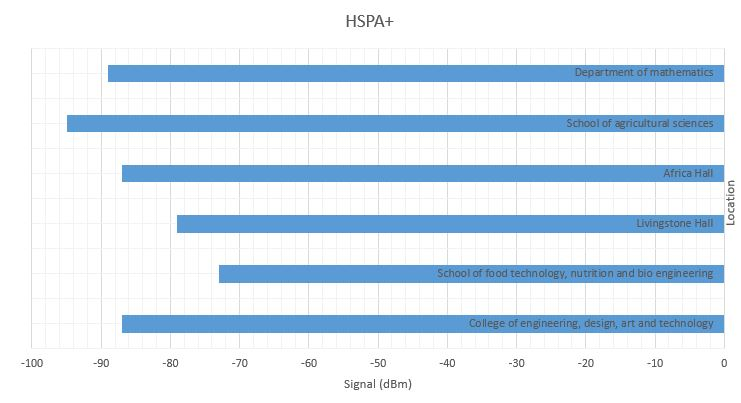
\includegraphics[width=\linewidth]{hspap.jpg}
  \caption{HSPA+}
  \label{fig:hspap}
\end{figure}

\begin{figure}
  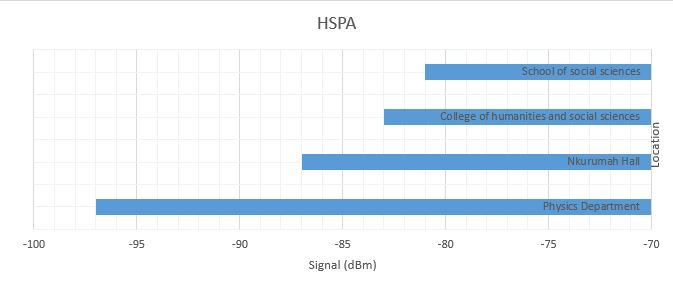
\includegraphics[width=\linewidth]{hspa.jpg}
  \caption{HSPA}
  \label{fig:hspa}
\end{figure}

\begin{figure}
  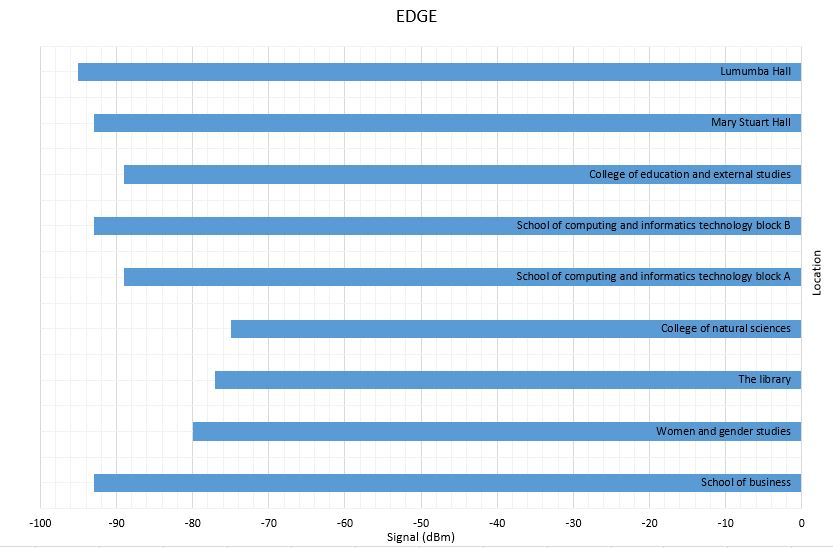
\includegraphics[width=\linewidth]{edge.jpg}
  \caption{EDGE}
  \label{fig:edge}
\end{figure}

\begin{figure}
  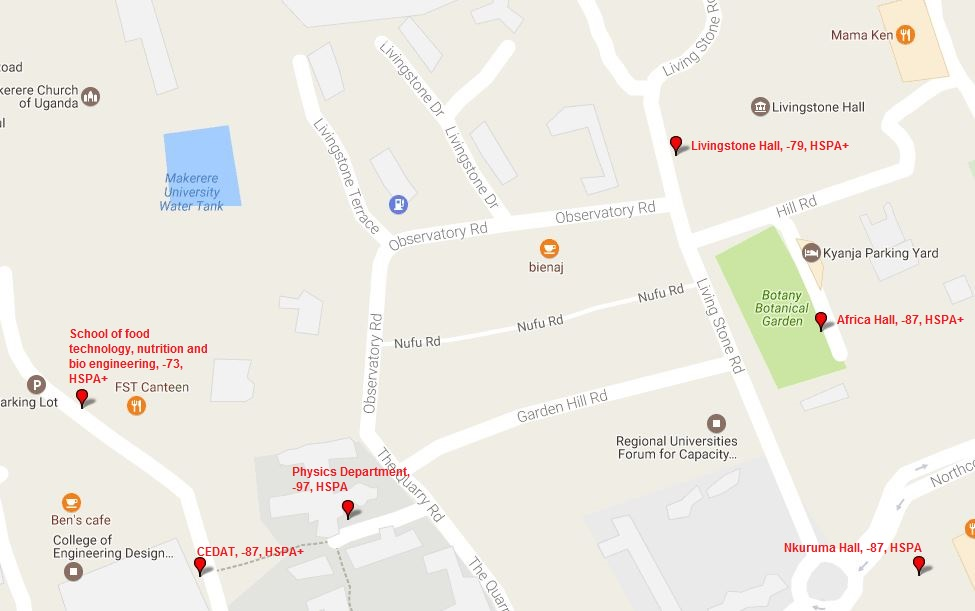
\includegraphics[width=\linewidth]{north.jpg}
  \caption{North part of the University}
  \label{fig:north}
\end{figure}

\begin{figure}
  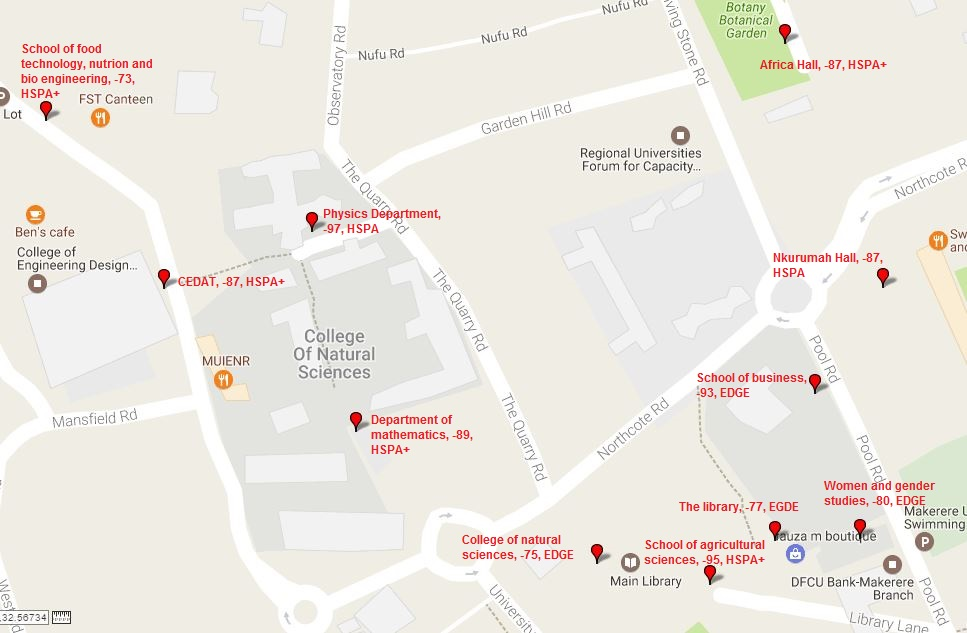
\includegraphics[width=\linewidth]{middle.jpg}
  \caption{Middle part of the University}
  \label{fig:middle}
\end{figure}

\begin{figure}
  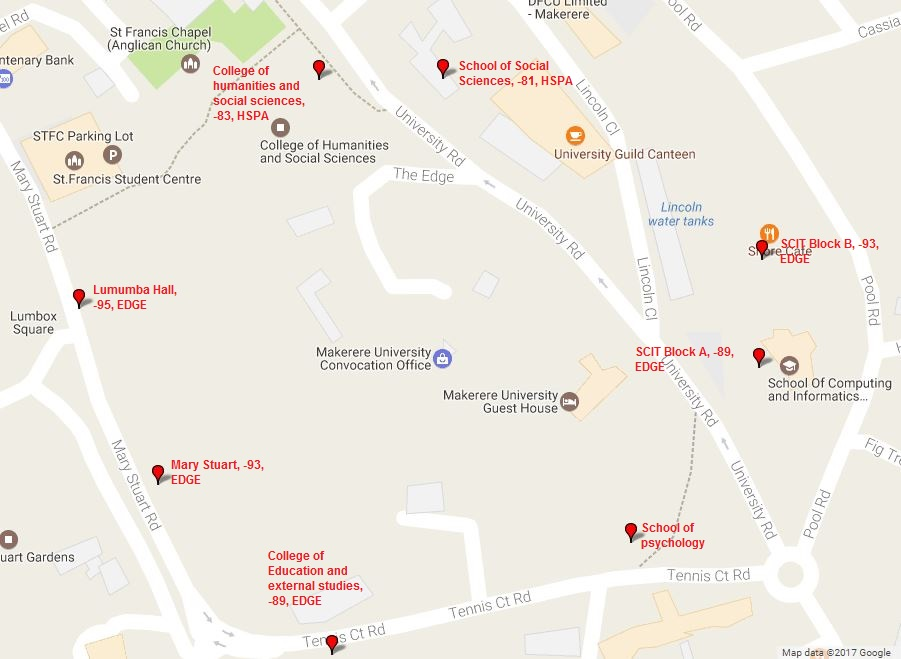
\includegraphics[width=\linewidth]{south.jpg}
  \caption{South part of the University}
  \label{fig:south}
\end{figure}

		\subsection{Discussion}
			\subsubsection{Network technologies}
				\paragraph{HSPA}
\cite{key:3} HSPA is the combination of HSDPA and Enhanced UL – also called HSUPA.  The maximum channel rate for Enhanced UL is 5.8 Mbps, with a peak data rate of 5.4 Mbps. The maximum channel rate for HSDPA is 14.4 Mbps, with a peak user data rate of 13.4 Mbps (on MAC level), compared with a maximum user data rate of 384 kbps.

				\paragraph{EDGE}
\cite{key:4} EDGE (Enhanced Data rates for Global Evolution), or Enhanced GRPS. Download speeds of 120Kbps to 384Kbps placed EDGE as an early pre-taste of 3G, although it was labeled 2.75G by industry watchers.

			\subsubsection{Mobile Phone Signal}
A mobile phone signal (also known as reception and service) is the signal strength (measured in dBm) received by a mobile phone from a cellular network (on the downlink). Depending on various factors,such as proximity to a tower,any obstructions such as buildings or trees, etc.,this signal strength will vary. Most mobile devices use a set of bars of increasing height to display the approximate strength of this received signal to the mobile phone user.  On Android devices, tools like Network Signal Info\cite{key:5} can directly show the signal strength (in dBm). Signal is usually measured in dBm. dBm is the power ratio in decibels of the radio power per one milliwatt. A signal of -60dBm is nearly perfect, and -112dBm is call-dropping bad. If you're above about -87 dBm, Android will report a full 4 bars of signal.\cite{key:6}

\section{Conclusion}
Mobile network distribution around the university is generally good with some exceptions of locations situated within the university unlike locations situated at the edge of the university.
			
\begin{thebibliography}{9}
\bibitem{key:1}
Guowang Miao; Jens Zander; Ki Won Sung; Ben Slimane (2016). Fundamentals of Mobile Data Networks. Cambridge University Press. ISBN 1107143217.
\bibitem{key:2}
Internet Usage Statistics [Online].  Available: http://www.internetworldstats.com/stats.htm
\bibitem{key:3}
HSPA [Online] Available: http://www.3gpp.org/technologies/keywords-acronyms/99-hspa
\bibitem{key:4}
EDGE [Online] Available: http://www.3gpp.org/technologies/keywords-acronyms/102-gprs-edge
\bibitem{key:5}
"Network Signal Info - Android Apps on Google Play". Retrieved 2016-06-29.
\bibitem{key:6}
How To Measure Cell Signal Strength on Android Phones [Online] Available: http://www.tested.com/tech/android/557-how-to-measure-cell-signal-strength-on-android-phones/
\end{thebibliography}

\end{document}